\documentclass[a4paper]{article}
\usepackage{graphicx}
\usepackage{tabularx}

% $Id$

\title{Eprints Archive Software System Documentation}
\author{Robert Tansley \and Christopher Gutteridge}

\newcommand{\eprints}{\emph{Eprints}}


\begin{document}

\maketitle

\tableofcontents

\section{Introduction}

This document describes the workings of the Eprints archive software, and how it interacts with the other components to provide services.

What this document does not contain is an API specification. Nor does it contain detailed information about what each file in the distribution does. The code is richly commented; this information is by and large not duplicated in this document. Producing such a document would have delayed the \eprints\ release by weeks. The best way to learn about the system, and how to achieve something, is to look at the code, read the comments therein, and follow the code's example. The comprehensiveness of this document should improve over time.

Before I delve in, a short note about programming style. The code is designed to be viewed with a tab width of 3. Tabs are \emph{always} used for indentation. Indentation of eight spaces is far too much, and using a combination of spaces and tabs just causes problems.

In your site specific code, and especially if you're developing the core code itself, please follow the style of the existing code, and comment richly, to enable the \eprints\ software to be easily maintainable in the future.

\subsection{Further Help and Bug Reports}

Technical queries (\emph{not} bug reports) concerning the \eprints\ software should be sent to:

\begin{verbatim}
support@eprints.org
\end{verbatim}

General information queries should be sent to:

\begin{verbatim}
info@eprints.org
\end{verbatim}

If you suspect you have found a bug, or an error in the documentation, please check the bug reporting system at:

\begin{verbatim}
http://bugs.eprints.org/
\end{verbatim}

If the problem has not already been reported, submit a bug report to the system.

Suggestions for new features to add to the software (wishlist items) can also be submitted to the bug report system.


% $Id$

\section{Overview}

\eprints\ works by interacting with several other components, as shown in figure \ref{fig_components}. Most interaction occurs through a Web browser interface, though during installation and in rare circumstances some \eprints\ scripts are run from a command line.

\begin{figure}
\centerline{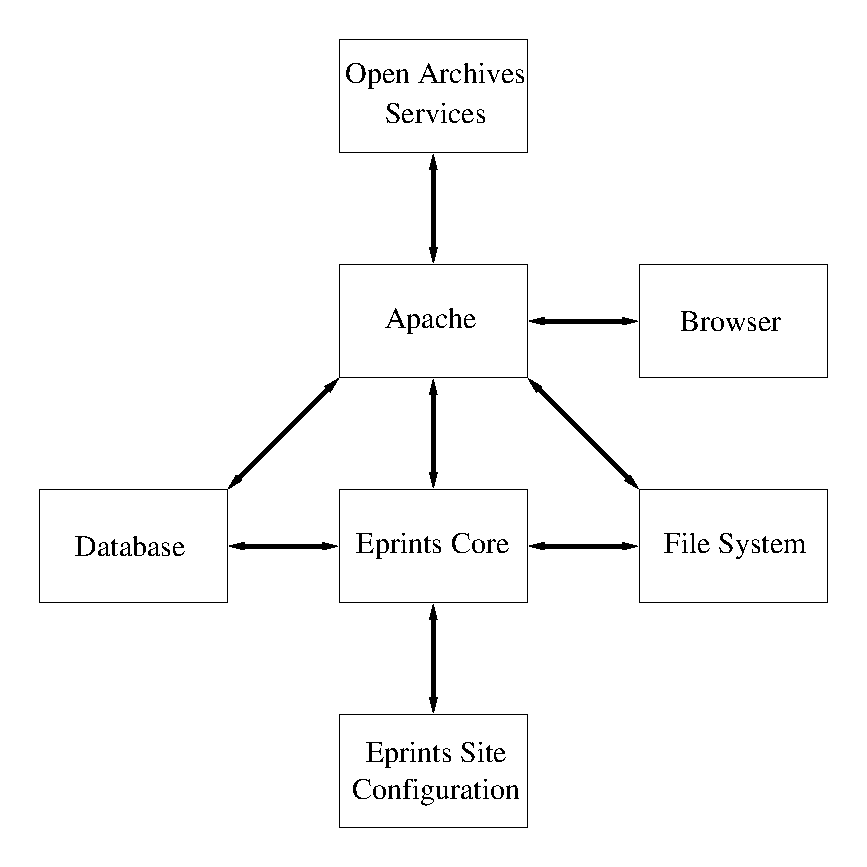
\includegraphics[width=3.5in]{images/components}} 
\caption{\label{fig_components} Overview of the Components of an \eprints\ archive}
\end{figure}

\subsection{Directory Structure}

This section lists and describes the directories in an installed \eprints\ system.

\begin{description}
\item[bin]

This directory contains various command line scripts. Some are used during installation and maintenance, some are invoked regularly via {\tt crontab} or equivalent, and one is invoked whenever an email message arrives at the automatic administration account.

\item[cfg]

Contains the plain text-based configuration files that constitute part of the site-specific portion of the \eprints\ archive. They contain information about what metadata to hold about each eprint and user, the initial subject hierarchy and templates for standard mails automatically sent to users.

\item[cgi]

Contains the Perl scripts that are invoked by the Apache WWW server. These scripts create those pages with dynamic content, for example search results and the eprint depositing interface. It is strongly recommended that you do not edit the contents of the scripts in this directory, since it will make upgrading the \eprints\ software rather difficult. You may wish to add further scripts; it is recommended that you name these carefully to avoid name clashes with any scripts that may be added to the core \eprints\ software in the future, for example by adding your own prefix {\tt my\_newscript}.

\item[html]

This directory is the document root for the Apache WWW server. All static files are stored under this directory. Note that the contents of this directory are managed entirely by the \eprints\ code, and its contents should not be manually edited. To manually add static files (e.g. image files or HTML documents) to the archive, use the {\tt static} directory and the {\tt generate\_static} script.

\item[html/documents]

This directory should contain symbolic links to areas eprints can be stored in. It must contain at least one before the system can run. See section \ref{eprint_storage} for further details. Note that while it is possible to simply create a subdirectory in which to store eprint files, this is not recommended since the contents of the {\tt html directory} should be considered volatile, but the eprint files themselves are not.

\item[perl\_lib/EPrints]

Contains the core \eprints\ Perl library files.  It is strongly recommended that you do not edit these files at all, since it will make upgrading the \eprints\ software extremely difficult.

\item[perl\_lib/EPrintSite]

Contains the Perl library files that constitute part of the site-specific portion of the software. These contain information that is difficult or inefficient to store in plain text-based configuration files. If and when you change or add functionality to the archive, it is strongly recommended that you put as much of the code as possible in this directory.

\item[openarchives]

Contains the old Open Archives subset of the Dienst software developed at Cornell University, with some minor modifications to work with the \eprints\ software. This code is invoked by the Apache WWW server to respond to Dienst requests, enabling the harvesting of metadata in the archive by Open Archives service providers. This protocol is no longer used by the Open Archives Initiative, but is included for the time being to allow \eprints\ archives to be harvested by service providers only supporting this old protocol.

\item[static]

Contains the static files (apart from the eprints themselves) that make up the \eprints\ WWW site. In the distributed version of \eprints\, these include a ``home page,'' some online help ages for users, the staff page menu and a general information page. However it is highly likely  that these will end up varying greatly from site to site. You can therefore add, remove and change as much as you like in this directory. However, it is recommended that if possible, you do not change the online help files (in the {\tt help} directory) since these have been designed to be site-independent, and will be kept updated with new capabilities and features in  new \eprints\ releases.

The {\tt generate\_static} copies the files in {\tt static}, including the directory hierarchy, to the {\tt html} directory. Non-HTML files are copied verbatim. HTML files are ``filled in'' with appropriate values in place of the placeholders, and given the site ``skin'' (look and feel) if appropriate.
\end{description}


\subsection{The {\tt html} Directory}
\label{eprint_storage}

The contents of the {\tt html} directory are controlled entirely by the software; you should not edit or add things directly. If you want to add an HTML page, graphic or other miscellaneous file to your site, add it to the {\tt static} directory and run {\tt generate\_static} (or {\tt update\_laf}.) The file will be added to the archive Web server.

In order to reduce processor load, and to enable search engines such as Google or AltaVista to index them, the ``Browse by Subject'' views and eprint abstract pages are generated once and then stored as ordinary {\tt .html} files.

You don't generally need to worry about abstract files; the core code updates these as necessary. If you make a change to the site configuration (e.g. the HTML ``skin'') you can force \eprints\ to regenerate all of the abstract files by running the {\tt generate\_abstracts} script. (The {\tt update\_laf} script will also do the same job, updating all other pages on the site at the same time.)

The ``Browse by Subject'' views are generated by running {\tt generate\_views} (or again {\tt update\_laf}). This should be done at least once a day; the automatic installer can install a suitable crontab for you. If your site has a lot of traffic you may wish the views to be generated more than once a day; this is easy to achieve by setting up a suitable crontab. Note that in the crontab you should run {\tt generate\_views}, and not {\tt update\_laf}, since the latter may regenerate a large number of pages and affect your server's performance.

\subsection{Eprint and Document File Storage}

When an eprint object is created, is it given an ID code, and a directory under {\tt html/documents} is created. The ID code is just a prefixed ordinal number; it holds no information about (say) the date it was created. The advantage of using a simple number scheme is that it gives the user a great deal of leeway when entering an ID code into the `view eprint' box; they do not need to remeber how many digits an ID code has to be for example. Given any unprefixed number the system can reason about which eprint the user is referring to.

When the eprint object is created, it will alphabetically scan each subdirectory, and the first subdirectory it finds with enough space will be used to store the new eprint and document files. The name of the directory for the eprint is worked out from its ID code. An eprint with the idcode {\tt ep12345678} will be in the directory:

\begin{verbatim}
12/34/56/78
\end{verbatim}

When the abstract pages of eprints are generated, the system gives the page the site skin ({\tt html\_head} and {\tt html\_tail} in {\tt SiteInfo.pm}), and calls the {\tt eprint\_render\_full} method in {\tt SiteRoutines.pm} to obtain the content of the page. The resulting HTML is stored in a file called {\tt index.html} in the eprint's directory.

Documents files stored with the eprint are stored in further subdirectories. A collection of document files pertaining to a single storage format have a separate document ID and are held in a separate directory. This ID is just the same as the eprint ID, with {\tt -00} appended for the first document format, {\tt -01} for the second, and so on.

For example, the eprint {\tt ep12345678} might have two associated document storage formats: A collection of HTML files and a PDF file. In the file system, this might look like:

\begin{verbatim}
12/
   34/
      56/
         78/
            index.html
            ep12345678-00/
               article.html
               figure1.gif
               figure2.gif
            ep12345678-01/
               article.pdf
\end{verbatim}

Information about the files stored in each for each document storage format is not stored in the database; only the name of the file that is to be displayed first when the user wishes to view that format is stored. In the above example, that would be {\tt article.html} for document {\tt ep12345678-00}, and {\tt article.pdf} for document {\tt ep12345678-01}.


\section{\eprints\ Metadata Handling}

This section describes how metadata is specified, stored and accessed in the \eprints\ system.

Metadata fields in the \eprints\ system will be of one of the types listed in table \ref{table_metadata_types}:

\begin{table}
\begin{tabular}{|l|l|}
\hline
{\tt boolean}    & true or false \\
{\tt date}       & a date (day, month and year) \\
{\tt email}      & an e-mail address \\
{\tt enum}       & one of a specified set of values \\
{\tt eprinttype} & a type of eprint (generally only used by system) \\
{\tt int}        & integer value (unsigned) \\
{\tt multitext}  & (potentially) several lines of text \\
{\tt multiurl}   & several WWW site addresses \\
{\tt name}       & a person's name, or list of people's names \\
{\tt username}   & a person's eprints username, or list thereof \\
{\tt pagerange}  & a range of pages (or a single page) \\
{\tt set}        & none or more of a specified set of values \\
{\tt subjects}   & none or more subjects in the subject hierarchy \\
{\tt text}       & a short, single line of text \\
{\tt url}        & a WWW site address \\
{\tt year}       & a year \\
\hline
\end{tabular}
\caption{\label{table_metadata_types} Types of Metadata Field in \eprints}
\end{table}

When you specify what metadata fields the system should store for each user or eprint, you need to decide which of the above types should be used for each field. The system will then know for each field:

\begin{itemize}
\item how to render the input fields in HTML
\item how to store it in the database
\item how to retrieve and search it
\item how to display it
\end{itemize}

There are two ways in which these metadata fields may be specified. The first is a fairly verbose method, akin to an Apache {\tt httpd.conf} file, used in the configuration files. In some cases, it is necessary to specify a field in code. In this case, a second, more terse format is used. The format used in the configuration files is described first.

\subsection{Verbose Metadata Field Specification}

A field is specified in the general form:

\begin{verbatim}
<field fieldtag>
arg1 = val1
varg2 = val2
...
</field>
\end{verbatim}

Here's an example. To specify that you want an optional ``Title'' field containing no more than 40 characters:

\begin{verbatim}
<field title>
required = NO
type = "text"
displayname = "Title"
maxlength = 40
editable = YES
visible = YES
</field>
\end{verbatim}

Below is a second example, describing a field in which the user can select one of three values:

\begin{verbatim}
<field ispublished>
editable = YES
type = "enum"
visible = YES
displayname = "Status"
value unpub = "Unpublished"
value inpress = "In Press"
value pub = "Published"
help = "Please state here whether your deposit has been "
help = "published, is currently in the process of being "
help = "published (<strong>in press</strong>), or has "
help = "not been previously published."
</field>
\end{verbatim}

The various arguments and possible values are listed in table \ref{metadata_arguments}. Note that the field tag, which must be unique, short and contain no spaces, is given in the {\tt <field>} line and is used to refer to the field in all other configuration files and code.

\begin{table}
\begin{tabularx}{350pt}{|l|l|X|}
\hline
Argument           & Types it applies to   & Description \\
\hline
{\tt type}         & ALL                   & the type of field, from table \ref{table_metadata_types} \\
{\tt required}     & ALL                   & is the field required? (YES or NO) \\
{\tt displayname}  & ALL                   & the name of the field to display to the user. \\
{\tt editable}     & ALL                   & is the field editable by users (as opposed to purely staff members?) (YES or NO) \\
{\tt visible}      & ALL                   & is the field globally visible? \\
{\tt help}         & ALL                   & a sentence or two of helpful text to display above the input box. This can be repeated, the values are just concatenated \\
{\tt displaylines} & {\tt multitext}, {\tt multiurl} & How tall the input box for the field should be \\
{\tt maxlength}    & {\tt text}            & maximum number of characters allowed (default=255, the maximum for the {\tt text} type) \\
{\tt value}        & {\tt enum}, {\tt set} & repeatable, specifies possible values for the field. Use in the form {\tt VALUE tag = "Displayed Version"}. \\
\hline
\end{tabularx}
\caption{\label{metadata_arguments} Arguments for Specifying Metadata Fields in a Metadata Schema}
\end{table}


\subsection{Terse Metadata Field Specification}

In order to allow some fields to be specified in-line in the code, there is an alternative, less human-readable way of specifying a metadata field. These consist of a single string, in the following form:

\begin{verbatim}
fieldname:type:misc arguments:displayable name:required?:
  editable?:visible?:indexed?
\end{verbatim}

Descriptions of each part are given below.

\begin{description}
\item[{\tt fieldname}] tag for the field (not the displayed name)
\item[{\tt type}] type of field, exactly as with the verbose specification method
\item[{\tt misc arguments}] these vary depending on the {\tt type}, and are described below.
\item[{\tt displayable name}] name for the field for displaying.
\item[{\tt required/editable/visible}] Correspond to the arguments for the verbose specification. A `1' means yes, a `0' means no.
\item[{\tt indexed}] This means the field will be indexed by the MySQL database. For this to be possible, the field must ALWAYS be non-null, and unique. It is up to the code to ensure that this is the case. For this reason, only fields specified in code can be indexed in this way; the core code cannot guarantee that a site-defined metadata field will always have a non-null value from the moment of record creation.
\end{description}

Miscellaneous arguments:

\begin{description}
\item[{\tt subjects}] Just a number, 0 or 1, indicating whether or not more than one value can be selected. If the number is 0, only one value can be selected.
\item[{\tt multitext}, {\tt multiurl}] Just a number, indicating how many lines high the input box should be.
\item[{\tt enum} and {\tt set}] The values the field may be set to. Possible values are separated by a semicolons. Each possible value is specified as a tag for internal representation, and a displayable name. For example:

\begin{verbatim}
never,Never (Off);daily,Every Day;weekly,Every Week
\end{verbatim}

This means the field can have the value {\tt never}, {\tt daily} or {\tt weekly}, which are displayed as ``Never (Off)'', ``Every Day'' and ``Every Week'' respectively.
\end{description}
 
For example:

\begin{verbatim}
datestamp:date::Submission Date:1:0:1:0
\end{verbatim}

This specifies a date field internally called {\tt datestamp} and displayed to the user as ``Submission Date''. It is a required field, but is not editable. It is publically visible, but not indexed by the MySQL database.


\subsection{The {\tt MetaField} Class}

Regardless of which way the metadata field was specified, it is used to instantiate a {\tt MetaField} object. It is by looking at this object that the system works out how the field should be displayed, stored, searched and read from an HTML form. Thus, the verbose method is there purely to ease the process of configuring the metadata that \eprints\ will store.


\section{The MySQL Database}

This section describes how the MySQL database is used, and the tables created and maintained by the \eprints\ software.

\eprints\ creates and uses the following tables:

\begin{description}
\item[{\tt counters}]
Holds incremental counters used to create ID codes without danger of clashes.

\item[{\tt users}]
Hold user records.

\item[{\tt inbox}]
The user's workspace, containing metadata for eprints currently being deposited.

\item[{\tt buffer}]
Contains metadata for eprints that are in the submissions buffer.

\item[{\tt archive}]
This is the main one; contains the metadata for the eprints that have been accepted into the archive.

\item[{\tt documents}]
Contains information about the eprint document files (e.g. PDFs, HTML files), such as the format, and which file should be displayed first when the users wants to view that format. Note that document file information for all eprints (in the workspace, buffer and main archive) are all held in this table.

\item[{\tt subjects}]
Contains the subject hierarchy.

\item[{\tt subscriptions}]
Contains the subscription (automatic e-mail alerting service) information.

\item[{\tt deletions}]
Holds information about removed eprints, and their replacements, if they exist.
\end{description}

Most tables are created by reading the relevant metadata field specifications from the relevant Perl class. The {\tt users}, {\tt inbox}, {\tt buffer} and {\tt archive} tables have additional columns. These are read in from the site metadata configuration files {\tt metadata.*} in {\tt eprints/cfg}. The database tables must correspond to these configuration files in order for the software to be able to extract and store data in the database correctly. Thus, if one a configuration file is changed, the database must be changed to match, and vice versa.

Database access is performed using the {\tt Database.pm} module. This provides methods to create tables, and create, update and retrieve records.


\subsection{Metadata Storage}

Due to the fact that the metadata schema is completely configurable by individual sites, \eprints\ cannot store all of the data in third normal form. This section describes how each metadata field type is stored.

Table \ref{internal_reps} shows how each metadata field type is stored in the database. The may  all have the value {\tt NULL}, provided that the particular field is not a primary key or indexed field in the database. Site-configured metadata fields may not be indexed as the core code cannot guarantee that the value will always be non-NULL from the start.

\begin{table}
\begin{tabularx}{350pt}{|l|l|X|}
\hline
Field Type & Stored as MySQL Type & Internal Representation (MySQL \& \eprints\ code) \\
\hline
boolean    & SET('TRUE','FALSE') & `TRUE' or `FALSE' \\
date       & DATE                & {\tt YYYY-MM-DD} \\
email      & VARCHAR(255)        & as-is \\
enum       & VARCHAR(255)        & tag of the selected value \\
eprinttype & VARCHAR(255)        & tag of the eprint type \\
int        & INT UNSIGNED        & the number \\
multitext  & TEXT                & as-is \\
multiurl   & TEXT                & as-is \\
username   & TEXT                & {\tt :username1:username2: }  \\
name       & VARCHAR(255)        & {\tt :surname,firstname middlename:surname Jr., firstname,middlename:} \\
pagerange  & VARCHAR(255)        & {\tt xxx-yyy}, {\tt xxx-}, {\tt -yyy}, or {\tt xxx} \\
set        & VARCHAR(255)        & {\tt :tag1:tag2:tag3:} \emph{tags in alphabetical order} \\
subjects   & TEXT                & {\tt :tag1:tag2:tag3:} \emph{tags in alphabetical order} \\
text       & VARCHAR(255)        & as-is \\
url        & VARCHAR(255)        & as-is \\
year       & INT UNSIGNED        & {\tt YYYY} \\
\hline
\end{tabularx}
\caption{\label{internal_reps} Internal Representation of Metadata}
\end{table}

The {\tt name}, {\tt set} and {\tt subject} types would ideally be stored in extra tables; however this would greatly increase the complexity of the database and reduce the performance of searches. A particular advantage with storing names in this format is that alphabetical ordering by surname can be achieved by simple ordering in an SQL statement.

The methods in {\tt Database.pm} automatically escape relevant characters and so on when instructing and querying the database with SQL. This means that, for example, you don't have to worry about prepending double quotes with a backslash.


\subsection{Relationships}

\eprints\ doesn't actually do any {\tt JOIN}s. Each record in the database (whether an eprint, document storage format, subject or user) is represented by an object in Perl, and one calls appropriate methods to discover related items. For example, in order to retrieve the document storage formats that a user has deposited for a particular eprint, one calls the {\tt get\_all\_documents} method of the {\tt EPrints::EPrint} class.



\section{The Searching Mechanism}

\eprints\ also knows how to search each of the metadata field types in the database. In order to do this, for each format, it must:

\begin{itemize}
\item Be able to render, and process input from, an HTML form;
\item Internally hold and be able to store search terms, for the subscription mechanism and passing the search terms between methods in the code;
\item Transform this internal representation into SQL for querying the database.
\end{itemize}

This means that \eprints\ has very powerful search capabilities in that any metadata field can be searched with fine granularity. The main drawback is that there is no notion of ``relevance'' of results; records are either retrieved or not retrieved, and the ordering is based on (for example) primary author's surname.

It should be noted that the search capabilities provided by \eprints\ are intended only as a starting point, in order to make the software useful in isolation, before Open Archives compliant services become commonplace. In the very near future, more powerful search and linking engines will be able to provide far more sophisticated services, and operate over many archives at once.


\subsection{Searching Metadata Fields}

{\tt SearchField.pm} is used by can render HTML input boxes for, store and query individual metadata search fields. It can actually search several fields at once; just pass in an array of {\tt MetaField} objects to its constructor.

The {\tt make\_meta\_fields} method in {\tt SearchExpression.pm} can be used to make an array of {\tt MetaField} objects by just passing in their names separated by slashes. So you can call {\tt make\_meta\_fields} with:

\begin{verbatim}
title/abstract/keywords
\end{verbatim}

and pass the resulting array into the {\tt SearchField} constructor to make a search field that will search the {\tt title}, {\tt abstract} and {\tt keywords} fields at once. Note that the fields must all use the same HTML input, internal representation and SQL; see the following sections. So, for example, you can search a {\tt text} field and a {\tt multitext} field as one, but not a {\tt text} field and a {\tt date} field.

Details of how the system performs each of the above three tasks for each metadata field type are given below:


\subsubsection{{\tt boolean} fields}

\begin{description}
\item[HTML Form:] Rendered as a popup menu with three choices, ``No preference'', ``Yes'' and ``no''.

\item[Internal representation:] {\tt TRUE}, {\tt FALSE}, or NULL ({\tt undef in Perl}) for no preference.

\item[In SQL:] {\tt TRUE} or {\tt FALSE} if a preference is specified; condition left out if no preference.
\end{description}


\subsubsection{{\tt date} fields}

\begin{description}
\item[HTML Form:] Rendered as a text input field, accepting the internal representation directly.

\item[Internal representation:] One of:
\begin{itemize}
\item {\tt YYYY-MM-DD}: A single day
\item {\tt YYYY-MM-DD-}: Open range, from the given date forwards (inclusive)
\item {\tt -YYYY-MM-DD}: Open range, from the given date backwards (inclusive)
\item {\tt YYYY-MM-DD-YYYY-MM-DD}: Close range between the given dates (inclusive)
\end{itemize}

\item[In SQL:] Converted to a simple ``LIKE'' for single days, greater than/less than comparisons for open-ended ranges, and ``BETWEEN'' for a closed range.
\end{description}


\subsubsection{{\tt email}, {\tt multiurl} and {\tt url} fields}

\begin{description}
\item[HTML Form:] Rendered as a text input field, accepting the internal representation directly.

\item[Internal representation:] Simple text string

\item[In SQL:] Just search for any record where this field contains this string (i.e. {\tt \%search text\%}
\end{description}


\subsubsection{{\tt enum} and {\tt eprinttype} fields}

\begin{description}
\item[HTML Form:] Rendered as a selection list, containing all possible values (in their displayable form) and ``(Any)''. The user may select as many values as they like. If no value is selected at all, ``(Any)'' is assumed.

\item[Internal representation:] Colon-separated list of values, in internal representation form, for example {\tt value1:value2:value3}. Value is {\tt undef} if any value is accepted for the search (e.g. if the user clicked on ``(Any)'' on the HTML search form.)

\item[In SQL:] Each possible value becomes {\tt OR}'d in the {\tt WHERE} clause of the SQL query.
\end{description}


\subsubsection{{\tt multitext} and {\tt text} fields}

\begin{description}

\item[HTML Form:] 
Rendered as a text field, with a popup menu to the side indicating how the search terms should be used: ``Match all, in any order,'' ``Match any'' and ``Match as a phrase.'' The name given to this extra input field is {\tt fieldname\_srchtype} (e.g. {\tt title\_srchtype}.)

\item[Internal representation:] {\tt all}, {\tt any} or {\tt phr}, indicating ``Match all, in any order,'' ``Match any'' and ``Match as a phrase'' respectively, followed by a colon, followed by the search terms. For example

\begin{verbatim}
any:mind reasoning consciousness
\end{verbatim}

This will match any record containing any of the words ``mind,'' ``reasoning'' or ``consciousness.''

If no search terms have been entered the internal representation is {\tt NULL} in MySQL and {\tt undef} in the Perl code.

\item[In SQL:] Depending on what type of matching is to occur (``Match any'' etc.) the search terms are {\tt OR'd} into separate {\tt LIKE} terms. Each term has {\tt \%} appended and prepended so it may be matched anywhere within a field. The drawback of this is that in particular, entering search terms with small numbers of letters (e.g.\ ``the'' or ``a'') will retrieve too many records.

\end{description}


\subsubsection{{\tt set}, {\tt username} and {\tt subject} fields}

\begin{description}
\item[HTML Form:] Rendered as a list of possible values, with a popup menu on the right hand side from which the user can select ``Any of these'' or ``All of these.'' If the user selects ``Any of these,'' the search will retrieve any record which has any value the user has selected in the relevant field. If the user selects ``All of these'', a retrieved record must have all of the values the user has selecetd in the list.  The name of this extra input field is {\tt fieldname\_anyall}.

\item[Internal representation:] Colon-separated list of the tags the user has selected, followed by {\tt ANY} or {\tt ALL}, corresponding to the user's selection of the ``Any/All of these''popup menu. For example:

\begin{verbatim}
tag1:tag2:tag3:ANY
\end{verbatim}

This will retrieve records where the field has any one of the values {\tt tag1}, {\tt tag2} or {\tt tag3}.

\item[In SQL:] Each tag is turned into a {\tt LIKE "\%:tag:\%} clause. Multiple tags are then combined with {\tt AND} or {\tt OR}  in order to construct the SQL query.
\end{description}


\subsubsection{{\tt year} fields}

\begin{description}
\item[HTML Form:] Rendered as a text input field, accepting the internal representation directly.

\item[Internal representation:] One of:
\begin{itemize}
\item {\tt YYYY-}: A single year
\item {\tt YYYY-}: Open range, from the given year forwards (inclusive)
\item {\tt -YYYY}: Open range, from the given year backwards (inclusive)
\item {\tt YYYY-YYYY}: Close range between the given years (inclusive)
\end{itemize}

\item[In SQL:] Converted to a simple ``LIKE'' for single years, greater than/less than comparisons for open-ended ranges, and ``BETWEEN'' for a closed range.
\end{description}


\subsection{Search Expressions}

In addition to the individual search fields, other parameters can be set, either in code or by the user on an HTML form. These parameters, together with the search fields themselves, are known as a \emph{search expression}.

A search expression is represented by a {\tt SearchExpression} object (in the {\tt SearchExpression.pm} module.) In addition to the search fields themselves, it holds:

\begin{itemize}
\item The table in the database being searched
\item Whether a `blank' search is allowed; that is, can a search with all search fields left blank be performed? A search with all fields left blank will simply return the entire database table. Because of the probably impact on your server, you probably will not want to allow public searches like this, and this is the default behaviour. However, staff searches can retrieve an entire database table.
\item Whether records should satisfy \emph{all} search fields to be retrieved, or just one. Basically, this just means are the search fields {\tt AND}'d or {\tt OR}'d?
\item How the results should be ordered.
\item The default ordering of results.
\end{itemize}

The ordering is specified in terms of SQL, for example:

\begin{verbatim}
year DESC, authors, title
\end{verbatim}

This sorts results by descending {\tt year}, then {\tt authors}, then {\tt title}. The default order if {\tt ASC}ending or {\tt DESC}ending are not specified is ascending.

{\tt SearchExpression.pm} can also produce a text string which, at a later time, can be fed back into {\tt SearchExpression.pm} to recreate the same search. This technique is used by the subscriptions mechanism to store and retrieve user subscriptions.



\subsection{Interactive and Non-interactive Searches}

Search forms are rendered and handled by the {\tt SearchForm.pm} module. This in turn uses the {\tt SearchExpression.pm} module in order to construct the query. 

Hence, in code, you should use {\tt SearchForm.pm} if you are creating an interactive search form, and {\tt SearchExpression.pm} if your are handling a search purely in code (for example, for a tailored subscription service.) You should always use {\tt SearchExpression.pm} even if your search is only searching one field, since {\tt SearchExpression.pm} contains code to construct the SQL query as a whole.



\subsection{Search Forms}

{\tt SearchForm.pm} handles more or less everything to do with an interactive search, including rendering the form, receiving the user input, performing the search and presenting the results. Creating a customised search is trivial; see {\tt search} and {\tt adv\_search} in the {\tt eprints/cgi} directory are good examples.

You could also quite easily put a ``quick search'' button on your archive's front page using something like the following HTML:

\begin{verbatim}
<FORM METHOD="GET" ENCTYPE="application/x-www-form-urlencoded"
ACTION="http://foo.ac.uk/perl/search">
  Enter a search term: 
  <INPUT TYPE="text" NAME="title_abstract_keywords">
  <INPUT TYPE="hidden" NAME="title_abstract_keywords_srchtype"
    VALUE="all">
  <INPUT TYPE="submit" NAME="Search" VALUE="Search">
</FORM>
\end{verbatim}

Note the use of hidden fields to specify defaults. The search scripts will also use defaults for any values that are omitted from the form. In the above example, there is no ordering information, so the search will just use the site default.


\section{Versioning, Comments and Responses}

The \eprints\ software features the ability for people to deposit new versions of eprints in the archive. They do this by entering the ID code of the previous version into the relevant box in the depositing interface. This (automatically validated) ID code is then stored in the {\tt succeeds} field in the eprint's metadata record. ({\tt succeeds} is a core metadata field that is always present; there is no need to configure this in your site configuration.) No information is stored with the eprint being succeeded.

This usually results in a chain of versions, but may result in a `tree' of different versions. A set of linked versions of an item are refered to as a ``version thread.'' By default, only the user who deposited the eprint may deposit a later version and link it to the previous version.

This linking information is then used by the default configuration to display links to all versions of the eprint being viewed. The core code will automatically work out which abstract pages need to be updated; any eprint in the thread will have its abstract page re-rendered.

This version information is stored in the deletions table if an eprint is removed from the archive. The ``404 Not Found'' error document handler then uses this information to see if a missing document is in fact a previously removed document, and can then direct the user to a more recent version. Note: For this to work, the newer version of the eprint must be installed into the main archive \emph{before} the old version is removed.


\subsection{Comments and Responses}

Exactly the same techniques are used to link commentaries and responses. If a user is submitting an eprint that is a commentary on another eprint, or another eprint responding to such a commentary, they enter the ID code in the relevant box on the depositing interface. This is then stored in the {\tt commentary} field; again the {\tt commentary} field is always present and doesn't have to be added to your site configuration.

Trees of commentaries and responses are also displayed on the abstract pages of all relevant items in the default site configuration; you can of course remove this. Unlike the versioning trees, any user can submit a commentary on (or response to) another eprint, regardless of who deposited the original eprint. Information about commentaries and responses are lost (the tree is broken) if an eprint in the tree is removed.


\section{Open Archives Interoperability}

A vital component of the software is the interoperability component. Version 1.1 of the software is compliant with
the Open Archives Protocol 1.0.

Using the protocol, an \eprints\ archive can export several metadata sets. By default only Dublin Core metadata is exported.

Two methods in the {\tt SiteRoutines.pm} module are used to configure the metadata your instance of \eprints\ will export. The {\tt oai\_list\_metadata\_formats} method returns a hash, mapping short metadata format names to their XML namespaces. By default, this just returns a hash defined in {\tt SiteInfo.pm}:

\begin{verbatim}
%EPrintSite::SiteInfo::oai_metadata_formats
\end{verbatim}

Code in the {\tt oai\_get\_eprint\_metadata} in {\tt SiteRoutines.pm} is used to map the site's internal metadata set to these formats.

For version 1.1, the base URL of the Open Archives protocol will be:

\begin{verbatim}
http://your.eprints.server.edu/perl/oai
\end{verbatim}

More information on Open Archives is available from:
\begin{verbatim}
http://www.openarchives.org/
\end{verbatim}

More information on the Open Archives Protocol is available from:
\begin{verbatim}
http://www.openarchives.org/OAI/openarchivesprotocol.htm
\end{verbatim}




\section{Handling of E-mail}

The \eprints\ system must be able to send and receive e-mail automatically. E-mails received in the \eprints\ archive automatic account (known as the \emph{autoadmin} account) must be piped to the standard input of (a newly run) {\tt process\_mail}. It's a good idea to have your mail system setup such that bounced error messages and messages sent to mailing lists (spam) are filtered out, for example using a {\tt procmail} recipe.

When the software \emph{sends} a mail, it should appear that it has been sent from the human-read admin account, so that replies can be directed appropriately.

\eprints\ understands two types of email automatically:

\begin{itemize}
\item Mails with the subject {\tt newuser} are used to create new user accounts. If an account for the From: address of the message already exists, a reminder of the username and password are sent to that address. Otherwise, an account is created, and an introduction e-mail returned giving the user their username and password, and instructions on how to proceed.
\item Mails with the subject {\tt change email} and containing the lines:

\begin{verbatim}
USERNAME username
PASSWORD abcdef
\end{verbatim}

Provided that the username and password are valid, the e-mail address associated with that user account will be changed to the address in the From: line of the e-mail. The reason address changes are handled this way is that if a user entered an incorrect e-mail address into a box, you have no way of contacting them to correct it.

If a user wishes e-mail to be directed to an address they cannot send from, they need to contact the site administration, who can use the user search and editing facilities in the staff area to change the address for them.
\end{itemize}

If the email isn't recognised, a return is sent with instructions on how to use the \eprints\ automatic mail processing correctly. You can change the wording of this text, including the ``introduction to the archive'' and the ``email successfully changed'' by changing the {\tt template.*} files in the {\tt cfg} directory.

\section{Running \eprints\ for a Department}

It is not unlikely that you will want to run the \eprints\ software as an archive for papers, or other media,
produced by a department or group with a specific set of members.

Key modifications you may wish to make might be:

\begin{itemize}
\item Remove email based user registration.
\item Update the users table from your members database with a crontab entry.
\item Add one or more {\tt username (multiple)} fields to metadata of the items to associate them directly with members. A ``Local Authors Usernames'' field, for example.
\item Add that field to the advanced search.
\item Edit the .htaccess files to use Encrypted passwords
\end{itemize}

You should try and avoid editing the core files (those in bin, EPrints and cgi) as
these will be overwritten when you next upgrade.

We are planning more support for this in the next release, including example scripts
to import users and a method for building static ``view'' pages for each member.
This would mean that your members could link from their homepage to a page listing
all their papers (or whatever your archive archives).

\section{Scripted Importing of Data}

It's likely that you have a large amount of data in another database or format that you want to populate your \eprints\ database with. The \eprints\ Perl modules make this importing trivial.

The best place to find information about methods is in the comments in the source files themselves. To help you get started, a simple example importing script is given below.

\begin{verbatim}
#!/usr/bin/perl -I/opt/eprints/perl_lib
# Note: Important you change the -I parameter appropriately

use EPrints::Database;
use EPrints::EPrint;
use EPrints::Session;
use EPrints::User;


# The 1 makes this an offline script
my $session = new EPrints::Session( 1 );

# Make a user (if any "create" type function returns undef,
# there was an error)
my $bbs_user = EPrints::User->create_user(
	$session,
	"auto",
	"Automated Import User",
	"User" );

# Make an eprint
my $new_eprint = EPrints::EPrint::create(
	$session,
	$EPrints::Database::table_archive,
	$bbs_user->{username} );

# Fill out the fields
$new_eprint->{title} = "This is the title";
# This is the internal name format. Or you can use EPrints::Name
# module to handle it for you
$new_eprint->{authors} = ":Tansley,Robert:Harnad,Stevan:";

# Puts the changes in the database
$new_eprint->commit();


# Make a document file
my $document = EPrints::Document::create(
	$session,
	$new_eprint,
	"HTML" );

# If you think a recursive web suck will work (make sure it
# doesn't grab the whole site!)
my $success = $document->upload_url(
	"http://www.foo.ac.uk/Archive/blah.html" );

# or for more fine tuned uploading
open INPUT, "blah.html" or die "Error opening blah: $!\n";

$document->upload( \*INPUT, "blah.html" );
$document->set_main( "blah.html" );

# Put changes in database
$document->commit();

# Terminate the session
$session->terminate();
\end{verbatim}

\section{Customisation Examples}

In this section we will give a few examples of simple but useful
modifications to the files in {\tt /opt/eprints/perl\_lib/EPrintSite/ }.

\subsection{Listing All Files in a Format}

In this example we have a data format which has no "start file". Our example
format is "Multiple Images". It is for an archive which expects you to submit multiple versions of the same image in different formats - ie. a 10meg TIF, a 2meg TIF and a small JPEG. On the abstract page for this record we want to list and link to all the files in this format, not just the "start" file.

\par The code which creates the link to each format from the abstract page is
in {\tt SiteRoutines.pm} in the subroutine called {\tt eprint\_render\_full}.

\begin{verbatim}
$html .= "<A HREF=\"".$_->url()."\">$description</A><BR>";    
\end{verbatim}

If we replace this line with the following code we should get a list of all
files when displaying this format:

\begin{verbatim}
if ( $_->{format} eq "MULTIPIC" )
{                                                                             
	# MULITPIC: Multiple Images Format
	# Special display for this format.
	$html .="<P><B>Multiple Images</B></P><UL>";                         
	my %files = $_->files();                                                
	my $file;                                                               
	foreach $file ( sort keys %files )                                      
	{                                                                       
		$html .= "<LI><A href=\"".$eprint->url_stem() . $_->{docid} .   
                         "/" . $file."\">".$file."</A>\n";
	}                                                                       
	$html.="</UL>";                                                         
}                                                                             
else                                                                          
{                                         
	# Display a normal format
	$html .= "<A HREF=\"".$_->url()."\">$description</A><BR>";              
}         
\end{verbatim}

You will need to run {\tt /opt/eprints/bin/update\_laf} to have this take
effect on static pages. To make this take affect on pages generated on 
the fly (eg. Viewing item in submission buffer) you will need to restart
the webserver.




\end{document}
